
\documentclass{article}
%\usepackage[left=1in, right=1in]{geometry}
\usepackage{graphicx}
\usepackage{listings}

\title{Semester Project - SDN assisted DMM }
\author{Monia Chouaibi- Lucas Croixmarie}
\setcounter{tocdepth}{2}

\begin{document}


\maketitle
\newpage
\tableofcontents
\newpage
\part{Project Context and Environement}

Mobile communications systems revolutionized the way people
communicate, joining together communications and mobility. A long way
in a remarkably short time has been achieved in the history of
wireless.  Looking past, wireless access technologies have followed
different evolutionary paths aimed at unified target: performance and
efficiency in high mobile environment. Nowadays the trend is to
visualize the network.\\ 
Another challenge is the growing number of Internet-connected users,
devices and applications such as the pool of available addresses for
the original version of the Internet Protocol, known as IPv4, is being
rapidly depleted. The solution come with IPv6 protocol that uses
128-bit addresses and provides such a vast number of addresses that it
can only be expressed mathematically: 3.4 x. Ipv6 is not only a good
approach but also helps to :

\begin{itemize}

  \item Solve security issues throw IPSec, which provides
    confidentiality, authentication and data integrity.
  \item Simplify Network configuration throw address
    auto-configuration mechanism.
  \item Save the bandwidth because IPv6 supports multicast rather than
    broadcast.
  \item Reduce the size of routing tables and make routing more
    efficient and hierarchical.
  \item Simplify packet header makes packet processing more efficient.
  \item Support new services like VoIP.
\end{itemize}


In this section we will first understand the mobility management in
mobile IPv6 then in proxy mobile IPv6. After that, we will show the
limitations of those technologies to move to explain the concept of
distributed mobility management in the SDN context.

\newpage
\section{Mobility Management Standardized solutions}

Internet traffic has increased steeply in recent years, due in great
part to social platforms and peer-to-peer networks. In addition,
users' wireless access represents an ever-growing portion of such
demand, thus posing a paradigm shift in the flow of Internet
information, for which most deployed architectures are not prepared
for. This evolution in user traffic demand is tackled by a different
approach for IP mobility, called Distributed Mobility Management, that
is focusing on moving the mobility anchors from the core network and
pushing them closer to the users, at the edge of the network. So,
let's first focus on the way mobility is treated is mobile IPv6 and
then in proxy mobile IPv6.

\subsection{Mobile IPv6}

\subsubsection{Principle}

The figure below shows the  network components in mobile IPv6: 

\begin{figure}[h!]
  \centering
    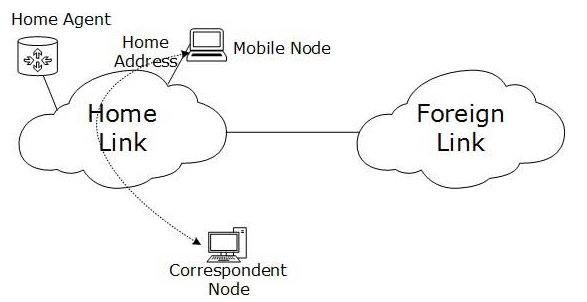
\includegraphics[scale=0.5]{reportPictures/figure1.png}
  \caption{Mobile IPv6 general overview}
\end{figure}


let's define each one of them:
\begin{description}
  \item[Mobile Node] \hfill \\ 
A node that can change its point of attachment from one link to
another, while still being reachable via its home address.
  \item[Correspondent Node] \hfill \\
A peer node with which a mobile node is communicating.  The
correspondent node may be either mobile or stationary.
  \item[Home Link] \hfill \\ 
This link is configured with the home subnet prefix and this is where
the Mobile IPv6 device gets its Home Address.
  \item[Foreign Link] \hfill \\
Any link other than the mobile node's home link.
  \item[Home Agent] \hfill \\ 
A router on a mobile node's home link with which the mobile node has
registered its current care-of address.  While the mobile node is away
from home, the home agent intercepts packets on the home link destined
to the mobile node's home address, encapsulates them, and tunnels them
to the mobile node's registered care-of address.
  \item[Home Address] \hfill \\ 
A unicast routable address assigned to a mobile node, used as the
permanent address of the mobile node.  This address is within the
mobile node's home link.  Standard IP routing mechanisms will deliver
packets destined for a mobile node's home address to its home link.
Mobile nodes can have multiple home addresses, for instance, when
there are multiple home prefixes on the home link.
  \item[Care-of Address] \hfill \\
A unicast routable address associated with a mobile node while
visiting a foreign link the subnet prefix of this IP address is a
foreign subnet prefix.  Among the multiple care-of addresses that a
mobile node may have at any given time (e.g., with different subnet
prefixes), the one registered with the mobile node's home agent for a
given home address is called its "primary" care-of address.

\end{description}


When a Mobile Node leaves its Home Link and is connected to some
Foreign Link, the Mobility feature of IPv6 comes into play. After
getting connected to a Foreign Link, the Mobile Node acquires an IPv6
address from the Foreign Link, this address is called Care-of
Address. The Mobile Node sends a binding request to its Home Agent
with the new Care-of Address. The Home Agent binds the Mobile Node’s
Home Address with the Care-of Address, establishing a Tunnel between
both. Whenever a Correspondent Node tries to establish connection with
the Mobile Node (on its Home Address), the Home Agent intercepts the
packet and forwards to Mobile Node’s Care-of Address over the tunnel
already established. The figure below shows the tunnel :

\begin{figure}[h!]
  \centering
    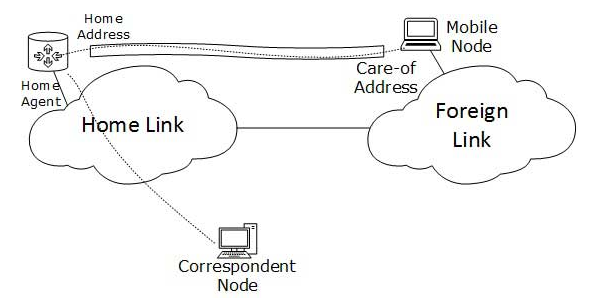
\includegraphics[scale=0.5]{reportPictures/figure2.png}
  \caption{Tunneling in Mobile IPv6}
\end{figure}

\newpage 

\subsubsection{Mobile IPv6 vs. Mobile IPv4}


The design of Mobile IP support in IPv6 (Mobile IPv6) benefits both
from the experiences gained from the development of Mobile IP support
in IPv4 (Mobile IPv4) , and from the opportunities provided by IPv6.
Mobile IPv6 thus shares many features with Mobile IPv4, but is
integrated into IPv6 and offers many other improvements. This section
summarizes the major differences between Mobile IPv4 and Mobile IPv6:\\
\newline
Mobile IPv6 operates without any support from local router (deployed
as a foreign agent ).\\
\newline
Security aspect no need to do a pre-arranged
security associations while moving It is expected that route
optimization can be deployed on a global scale between all mobile
nodes and correspondent nodes.\\
\newline
In Mobile IPv6 the home agent address discovery mechanism is dynamic
and returns a single reply to the mobile node. However in IPv4 the
directed broadcast approach is used and returns separate replies from
each home agent.\\
\newline
Most packets sent to a mobile node while away from home in Mobile IPv6
are sent using an IPv6 routing header rather than IP encapsulation,
reducing the amount of resulting overhead compared to Mobile IPv4.

\subsection{Proxy Mobile IPv6}

Proxy Mobile IPv6 (or PMIPv6, or PMIP) is a network-based mobility
management protocol standardized by IETF and is specified in RFC
5213. It is a protocol for building a common and access technology
independent of mobile core networks, accommodating various access
technologies such as WiMAX, 3GPP, 3GPP2 and WLAN based access
architectures. Proxy Mobile IPv6 is the only network-based mobility
management protocol standardized by IETF.

\subsubsection{components}

The figure 3 shows an Overview of PMIPv6 architecture: 

\begin{figure}[h!]
  \centering
    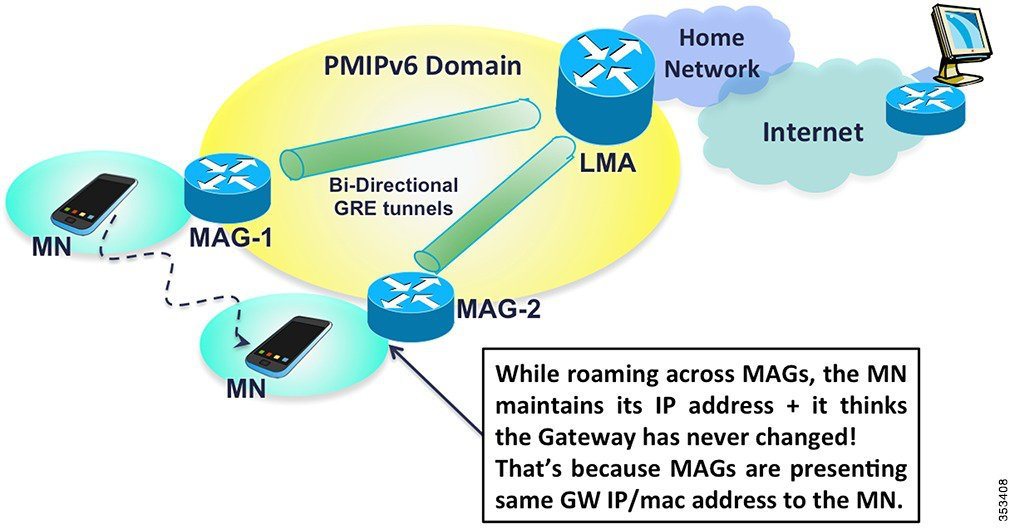
\includegraphics[scale=0.5]{reportPictures/figure3.jpg}
  \caption{PMIPv6 architecture}
\end{figure}


These are some definitions of network components : 

\begin{description}
  \item[Local Mobility Anchor (LMA)] \hfill \\ 
it is similar to HA in MIPv6.  It is the topological anchor point for
the mobile node's home network prefix(es) and is the entity that
manages the mobile node's binding state. LMA includes a binding cache
entry for each currently registered MN with MN-Identifier, the MN's
HNP, a flag indicating the proxy registration and the interface
identifier of the bidirectional tunnel between the LMA and MAG.
  \item[Mobile Access Gateway (MAG)] \hfill \\ 
Mobile Access Gateway is a function on an access router that manages
the mobility-related signaling for a mobile node that is attached to
its access link.  It is responsible for tracking the mobile node's
movements to and from the access link and for signaling the mobile
node's local mobility anchor.
\end{description}

\subsubsection{message exchanges}

The execution of the message flow of the overall operations in PMIPv6
is show in the figure below:

\begin{figure}[h!]
  \centering
    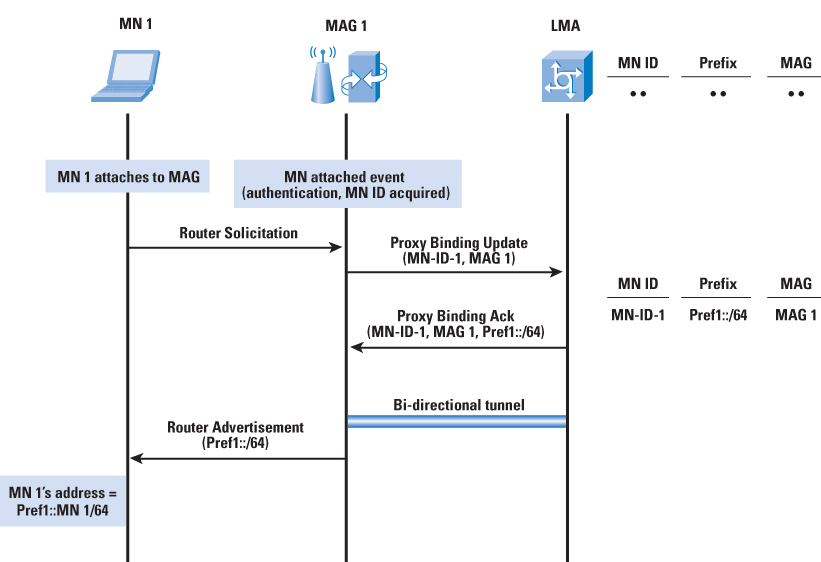
\includegraphics[scale=0.4]{reportPictures/figure4.jpg}
  \caption{Tunneling messages under PMIPv6}
\end{figure}

The MN attaches to the MAG that performs an authentication procedure
with a policy server using the MN's profile, which contains
MN-Identifier, LMA address and other related configuration parameters
before sending to the LMA a Proxy Binding Update (PBU) message on
behalf of the MN including the MN-Identifier. the LMA by his turn
replies with a Proxy Binding Acknowledgment (PBA) message including
the MN's HNP.\\
\newline
With this procedure the LMA creates a Binding Cache Entry (BCE) for
the MN and a bi-directional tunnel between the LMA and the MAG is set
up Then the MAG sends Router Advertisement message to the MN on the
access link advertising the MN's HNP as the hosted on-link-prefix. On
receiving this message, the MN configures its interface either using
stateful or stateless address configuration modes. Finally after
obtaining the address configuration in the Proxy Mobile IPv6 domain,
as the mobile node moves and changes its point of attachment from one
mobile access gateway to the other, it can still continue to use the
same address configuration.  As long as the attached access link is in
the scope of that Proxy Mobile IPv6 domain, the mobile node will
always detect the same router advertising itself as default-router and
advertising the mobile node's home network prefix(es) on each
connected link.

\subsection{Limitations of those Techniques}

PMIPv6 and Mobile IPv6 was promising technologies but in the recent
years user profile has changed , so that finding a solution for
mobility of MN is one of the most critical criterion of selection in
the operator perspective . Looking for an alternative resolution is
due to these facts :
\begin{itemize}

  \item 
Inter-domain handover is not supported .When the mobile node moves to
another PMIPv6 domain the on-going sessions cannot be maintained.
  \item 
Centralized mobility management is simple to be implemented because
the central anchor can follow the user movements by simply re-routing
the packets over tunnels created with the access router where the
mobile node is currently connected.  But the mobility anchor
represents a single point of failure, it poses scalability issues and
can lead to non optimal routing policies.
  \item  
Handover latency problem : It is known that, compared to PMIPv6, MIPv6
has inferior performance in handover latency . The heaviest
contribution to the handover latency of MIPv6 is made mainly by the
binding signaling delay. Unlike PMIPv6 and MIPv6 the routing update
procedure may cause a large delay.
  \item  
Hierarchical architecture of mobile and cellular networks forces the
user traffic to go through all network parts up to the core where key
entities are deployed to function as border IP gateways and mobility
anchors.
\end{itemize}

To overcome these limitations many solutions where proposed thus
Distributed mobility management DMM which aims to designing a flat
mobile architecture that enables enhanced access to IP services and
built-in support for mobility and heterogeneous radio access
technologies. The DMM framework envisions an all-IP infrastructure
where users’ data flows are routed through the optimal path,
exploiting multiple anchors points and deployment of IP services
closer to the users without requiring complex dedicated support from
the mobile nodes. Moreover a wise assignment of IP addresses to the
mobile nodes according to the available services for that user
provides a mobile operator with the flexibility to handle users’ data
traffic according to an extended set of policies. All of these
advantages combined with an intelligent network architecture that
distinguishes between the data plan and the control plan messages can
result in quicker provisioning and configuration of network
connections, high system performances, simplified networking as well
as the deployment of new protocols and applications. This approach is
called SDN-based DMM solution that we will introduce in the following
chapter.

\section{DMM Solutions}

\paragraph{Introduction}
Software-defined networking (SDN) is an approach to computer
networking that allows network administrators to manage network
services through abstraction of lower-level functionality. This is
done by decoupling the system that makes decisions about where traffic
is sent (the control plan ) from the underlying systems that forward
traffic to the selected destination (the data plane). The inventors
and vendors of these systems claim that this simplifies networking.\\
\newline
Let's see the architecture of the software defined network then we
will explain the distributed mobility management combined with this
solution.

\subsection{SDN general idea and scheme}

%\subsubsection{general presentation of SDN concept}

The figure below we can see the architecture of software defined network :

\begin{figure}[h!]
  \centering
    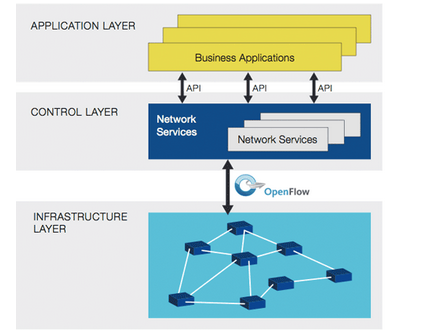
\includegraphics[scale=0.5]{reportPictures/figure5.png}
  \caption{SDN architecture}
\end{figure}

SDN decouple the data and the control plan. Actually, in SDN there is
three layers :

\begin{description}
  \item[The infrastructure layer] \hfill \\ 
SDN don't make restrictions on this layer. Transport of packets from
the eNB to mobile core network takes place over so called mobile
backhaul that makes use of all kinds of transmission and packet
transport technologies such as Ethernet, Carrier Grade Ethernet,
IP/MPLS and MPLS-TP. The physical layer in the backhaul networks uses
Fiber, Radio, and copper based links. The physical links are either
owned by the mobile operator or leased from another operator. An
incumbent mobile operator may share its infrastructure with different
types of mobile virtual operators. This approach helps to reduces the
costs of the radio network to the mobile operator and adds capacity
for the end user benefit.
  \item[Control layer] \hfill \\ 
Mainly we speak here about the SDN controller which is the brain of
the network . It contains a collection of “pluggable” modules that can
perform different network tasks. Some of the basic tasks including
inventorying what devices are within the network and the capabilities
of each, gathering network statistics, etc. Extensions can be inserted
that enhance the functionality and support more advanced capabilities,
such as running algorithms to perform analytic and orchestrating new
rules throughout the network.
  \item[Application layer] \hfill \\ 


\begin{description}
  \item[Mobile Backhaul Scaling] 
Manage and optimize the provision of backhaul connections from the
base stations to the Access App.
  \item[Mobility Management] 
When a mobile device moves the rule in mOFS for the device needs to be
modified and a new rule may need to be created in the new eOFS. If the
new eNB is under the same eOFS as the previous one, then it is enough
to modify an existing rule in the eOFS. We also need to take care of
balancing the load across the alternative paths between an eNB and a
particular mOFS. The Mobility Management App chooses the path for a
device. For the load balancing decision it needs input from network
Monitoring App.
  \item[Access App]
It aims to assign the IP address for the mobile device .
  \item[Secure Service Delivery App] 
It helps to secure the process of service delivery and maximally
benefiting from the economies of scale of cheap switches and generic
hardware for control processing. The minimum goals of the service
delivery network are to eliminate all source address spoofing and
DDoS.
\end{description}

\end{description}


Software-Defined Networking (SDN) is an emerging architecture that is
dynamic, manageable, cost-effective, and adaptable, making it ideal
for the high-bandwidth, dynamic nature of today's applications. This
architecture decouples the network control and forwarding functions
enabling the network control to become directly programmable and the
underlying infrastructure to be abstracted for applications and
network services.  SDN requires some method for the control plane to
communicate with the data plane. One such mechanism, OpenFlow, is
often misunderstood to be equivalent to SDN, but other mechanisms
could also fit into the concept.\\
\newline
So finally SDN, network administrators can program the behavior of
both the traffic and the network in a centralized way, without
requiring independently accessing and configuring each of the networks
hardware devices this can be helpful to cope with mobility
issues. Distributed mobility management come as a new approach to
concertize this in the context of IP mobility.


\subsection{DMM protocol presentation}

\paragraph{Introduction}
SDN allows allows for quicker provisioning and configuration of
network connections. So, network administrators can program the
behavior of both the traffic and the network in a centralized way,
without requiring independently accessing and configuring each of the
networks hardware devices. Also, this simplifies networking as well as
the deployment of new protocols and applications. In addition, by
enabling programmability on the traffic and the devices, an SDN
network might be much more flexible and efficient than a traditional
one. SDN-DMM based solution exploit these advantages to built a
promising solution that:\\
\newline
Cope with mobile traffic increase.  Distribute Mobility management
functions to multiple locations.  Serves Mobile node in any of these
networks by a closest mobility function.

\subsubsection{Components of the architecture}

The main component of the distributed mobility management are :

\paragraph{The network controller}
It is responsible to configure the nodes in the
network via a common application programming interface (API), namely
Southbound API which can be used by an external software application
to program the forwarding plane of network devices. In our solution,
it configures the forwarding rules on access routers (the DMM-GWs)
using OpenFlow 1.3 API

\paragraph{DMM-GWs}
It's a simple device mainly to forward packets , redirect traffic and
store some informations\\
\newline
the figure below shows the DMM -SDN based solution : 

\begin{figure}[h!]
  \centering
    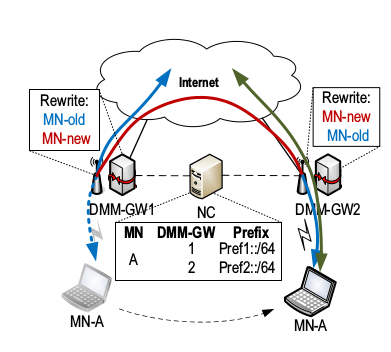
\includegraphics[scale=0.5]{reportPictures/figure6.png}
  \caption{DMM component}
\end{figure}

\subsubsection{Description of message exchanges}
Upon the MN's attachment to a cMAR, an IPv6 global prefix belonging to
the MAR's prefix pool is reserved for it (Pref1).  The prefix is sent
in a PBU with the MN's Identifier (MN-ID) to the CMD, which, since the
session is new, stores a Binding Cache Entry containing as main fields
the MN-ID, the MN's prefix and MAR1's address as Proxy-CoA. The CMD
replies to MAR1 with a PBA indicating that the MN's registration is
fresh and no past status is available.MAR1 sends a Router
Advertisement (RA) in unicast to the MN including the prefix reserved
before, that can be used by the MN to configure an IPv6 address (e.g
with stateless auto-configuration). The address is routable at the
MAR, in the sense that it is on the path of packets addressed to the
MN.\\
\newline
The figure below explains the whole procedure:

\begin{figure}[h!]
  \centering
    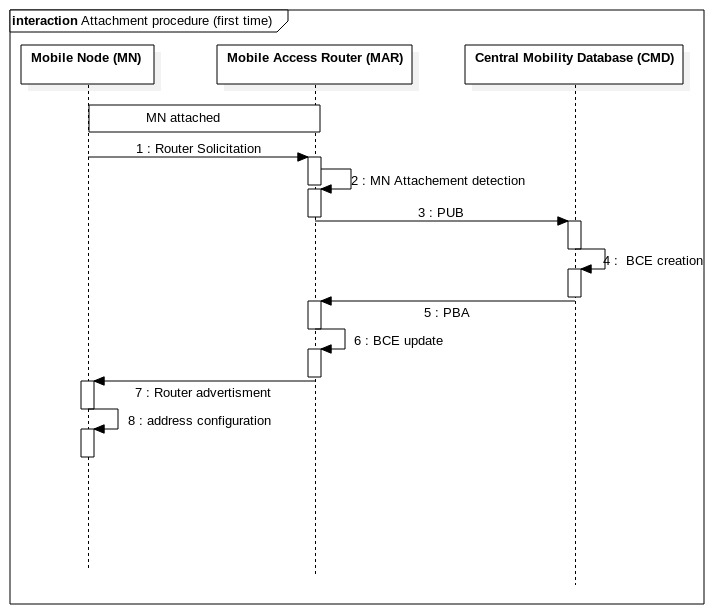
\includegraphics[scale=0.5]{reportPictures/figure7.jpg}
  \caption{Attachment procedure}
\end{figure}

let's see now the component of each message : \\
\newline

\begin{description}
  \item[MN attached]
After the Random Access procedure, if the MN is not already attached
to the network it has to do so by initiating the attach procedure.
  \item[Router solicitation]
The mobile node, MN, attaches to MAR which is responsible for
allocating the MN-HNP, the MAR contains data structure to store the
association of a network prefix and a mobile interface identifier.
  \item[MN attachment detection]
MAR allocates and advertises HNP and updates MN's mobility session up
to the database.
  \item[PBU]
A request message sent by the MAR to the CMD witch contains the MN-ID
and the HNP prefix.
  \item[BCE creation]
Update the cache. It Allocate MN-HNP(s)
  \item[PBA] 
A reply message sent by the CMD to a Proxy Binding Update message that
it received from the MAR.
  \item[BCE update] 
Setup BCE and Tunnel
  \item[Router advertisement] 
The mobile node can initiate and maintain data transport sessions
(with CN), using IP addresses derived from HNP, in a standard way
while it remains attached to MAR.
\end{description}


When a MN is moving away from the area covered by one MAR node and
entering a new area covered by another MAR, the handover process is
performed as shown in Figure below and the on going session is
transferred to the second MAR in order to avoid session termination
when the MN gets out of the range of the first MAR.\\
\newline 
When the MN enters the new MAR domain, initial attachment process is
performed and the MN gets the new IPv6 address which will be used for
new communication sessions to be started from now on. In the meantime,
the on going session keeps using the old IPv6 address that was gotten
from the previous MAR node that the MN visited when the session
started.\\
\newline
After detecting the approach of the MN, the new MAR allocates a new
HNP and creates a PBU message that includes the MN\_ID and the
allocated HNP and sends it to the CMD. When the CMD receives the PBU,
it uses the MN\_ID as a key to search the BCE table. The matched entry
is updated and becomes the form of {MN\_ID : (old\_HNP, old\_MAR\_ip)
  : (new\_HNP, new\_MAR\_ip)}. After updating the BCE entry, the CMD
replies to the new MAR with the PBA message that contains the
information about old MARs, {MN\_ID : (old\_HNP, old\_MAR\_ip)}. At
the same time, The CMD sends to the old MAR the PBU message with the
information of {MN\_ID : (old\_HNP, new\_MAR\_ip)}.\\
\newline
When receiving the PBA message, the new MAR node inserts the
information of {MN\_ID : (old\_HNP, old\_MAR\_ip)} into the BU(Binding
Update) list and establishes a tunnel to the old MAR. In the meantime,
the old MAR node that is receiving the PBU message from the CMD node
updates the BCE table entry by using the information of {MN\_ID :
  (old\_HNP, new\_MAR\_ip)} and establishes a tunnel to the new MAR
and replies to the CMD with the PBA message. \\
This can be shown through the figure 8.

\begin{figure}[h!]
  \centering
    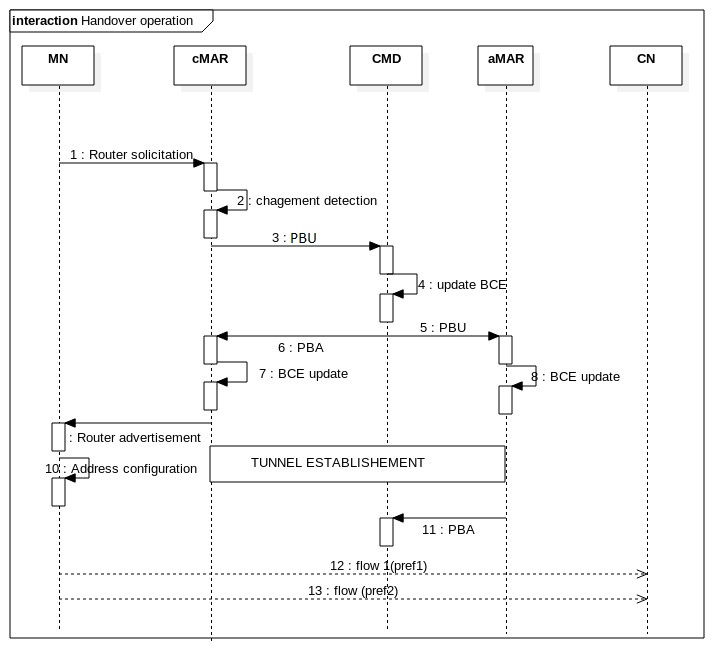
\includegraphics[scale=0.5]{reportPictures/figure8.jpg}
  \caption{Tunneling under DMM}
\end{figure}

\begin{description}
\item[CMAR]Correspondent Mobile Access Router
\item[CMD]Control Mobility Database 
\item[Router solicitation] The mobile node MN attaches to MAR which is
  responsible for allocating the MN-HNP. By sending this message the
  mobile node declare its presence and asks for the network
  information to configure its parameter.

\item[BCE creation]delete the sentence It Allocate MN-HNP(s).     
\end{description}

\newpage

\part{Project tools}

In order to implement the Distributed Mobility Management SDN oriented
previously described, several tools are required. We first need a SDN
protocol implementation, then a way to emulate a SDN compatible
network and finally a framework for the SDN controller.

\section{OpenFlow}

\subsection{Presentation}
OpenFlow is a communication protocol between the controller and the
switches in a SDN oriented network. Switches use it to report the
events they meet (e.g packet reception) to the controller, where all
the network intelligence is centralized. Then using this protocol the
controller sends to switches actions that have to be taken.

\subsection{The concept of flows}
OpenFlow formalizes the idea of orders pushed to switches by the
controller in introducing the concept of flows, indeed a flow is
composed by a set of fields set to certain values, those fields
correspond to the ones that compose the structure of the packets
exchanged between nodes, over the network. A elementary networking
action is join along the field set, it can be for example 'forward to
this interface'.\\
\newline
The controller as the brain of the network must have to tell to
switches what to do and when, then that is now that the structure of
flow is relevant : to transmit its order, the controller sends flows
with a set of fields set to match a specific kind of packet, exactly
like a firewall rule (for example type=ICMP, addr\_dest=198.168.1.12)
and with a action set to the action the controller wants the
recipient of the flow to do whenever it receives this kind of
packet.\\
\newline
With this approach switches get progressively autonomous, the more
they are instructed by flows from the controller, the less they refer
to it. Flows have a Lifetime and the controller can modify or even
delete them after their submission.  There are two ways of pushing
flows to switches, the first one is proactive and consists in
providing all the knowledge (i.e a complete set of flows) that
switches need when the network initializes.  The second method
is reactive : when a packet reaches a switch and doesn't match any
received flow, the switch asks the controller what to do with it, in
response the controller sends a flow matching the packet.

\subsection{Flow organization}
Inside switches, flows are organized into tables and are affected with
a priority level that defines the way they are ranked in the
table. For every packet received the switch scans linearly the flow
table, executes the action of the first matching flow and stops there.\\
\newline
If the switch reaches the end of the flow table without having found
any matching flow it reports it to the controller, but moreover a
default entry policy can be defined for the table, this is a way to
define a default behaviour for switches.\\
\newline
It is important to have in mind that when a switch is waiting for a
flow from the controller to know what to do with a packet just
received, if no default behaviour is set, the pending packet and the
similar next ones are lost until the flow is installed on the switch,
buffering mechanisms can be set up to avoid those losses.\\
\newline
As flows may have different purposes and as the user may want to scan a
first set of flows before a second one, multiples tables can be
used. They are ranked according to their identifier and can be bound
one after the other one so that different purposes flows are not mixed
up. It is not possible for the flow scanning process to loop over the
same table of to jump to a table with a lower identifier, it's a one
way scan.

\subsection{Punctual order}

The advantage of pushing flows is that the controller is only
solicited once by the switch to know it what to do with a specific
kind of packet. But there are some cases for which the user wants the
switch to keep the controller informed of the reception of the
same kind packets. To do so the controller doesn't reply to the switch
in providing him a flow but an individual elementary order, like a
flow only with the action part. Therefore switch performs the order and its
table doesn't change and then it will keep asking to the controller
what to do with this kind of packet.\\
\newline
When the switch requests the controller for an action to perform it
joins in the OpenFlow message the message that has made it send the
request. Then if the controller replies with a punctual order it also
joins the packet in the response so that the provided action can be
performed on the packet itself, and this way packet is not lost but
just delayed.

\section{Mininet}

\subsection{Presentation}
Mininet is a network emulator, it allows to create realistic virtual
network running switch and application code on a virtual
machine.\\
\newline
Mininet makes easy to virtualize hosts, switches, links, and
controllers and makes a single system looks like a complete network
because the most part of their behavior is similar to discrete
hardware elements.  The figure below shows the hierarchy of the
network building :

\begin{figure}[h!]
  \centering
    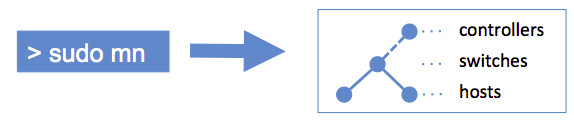
\includegraphics[scale=0.5]{reportPictures/figure9.png}
  \caption{Mininet basic elements}
\end{figure}

\subsection{Advantages and limitations}

Mininet is simplified tool that get configured from a python script,
then it is possible to design any kind of network with which the user
can dynamically interact through a Command Line Interface and then can
modify it at run-time.

Mininet suits particularly well SDN oriented networks as it provides
the envelop for the controller application, then the controller code is just
bound to it whatever its framework is. Messages between controller and
Mininet go through the local loop and hopefully, Mininet is compatible
with OpenFlow1.3.

The only problem met with Mininet is how complex it is to make the
topology change at run-time through the command line interface.

\section{Ryu}

\subsection{Presentation}
Ryu is the SDN framework used for the implementation of our solution,
it's python based, very flexible and embeds quite a lot of options
published by an active developer community. Writing a SDN controller
above Ryu is relatively easy as the framework abstracts all the
configuration and the interaction with OpenFlow then user just has to
tell what has to be done when a certain type of packet is received by
a certain switch.  Here is how it is located on a application stack:

\begin{figure}[h!]
  \centering
    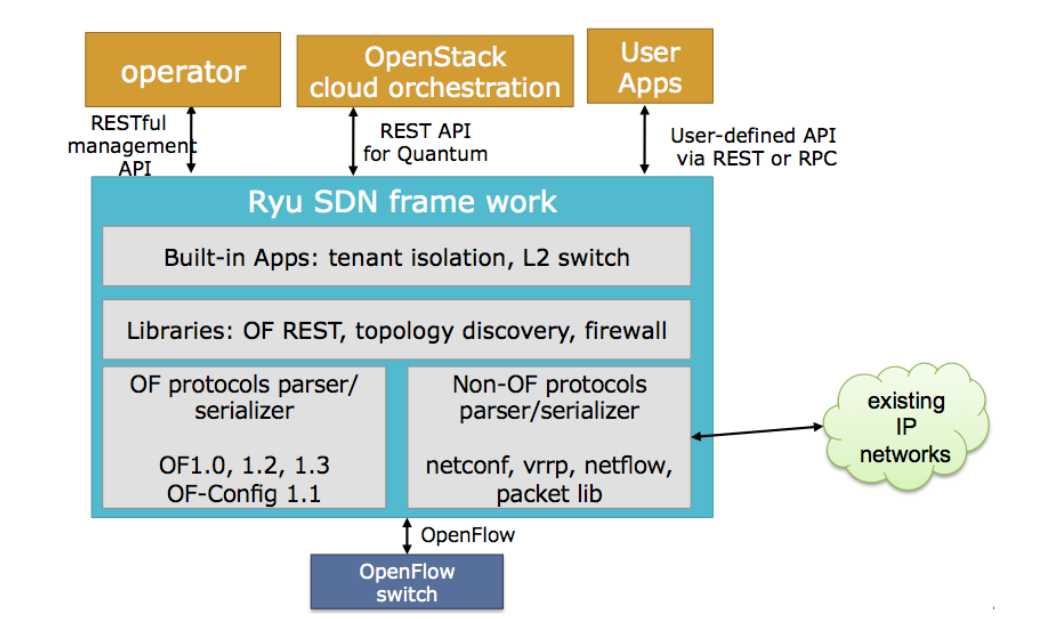
\includegraphics[scale=0.3]{reportPictures/ryu_layers.png}
  \caption{Ryu Architecture}
\end{figure}

\newpage 

\subsection{Comparison with other frameworks}
SDN controller frameworks are only a few and they are all very young,
all written in different languages. The first one is Open DayLight
comes from a consensus of several IT companies as it's running on a
Java Virtual Machine, it allow user to use Java Libraries. The problem
of this controller is that it's not handling IPv6 and is still stuck
to IPv4 then it can't be use for our project. Another python based
framework is POX but it also suffers from the same problem. Trema is a
framework that handle IPv6 addresses but it is still very young and
poorly documented.\\
\newline
This aim of this little part is mainly to say that SDN frameworks are
evolving fast, we have chosen Ryu because at this time it seems to be
the one that suits the most our project, but in few months it would be
maybe better to migrate the controller implementation under Open
DayLight framework to benefit its strong support.

\subsection{Ryu available resources}

A relatively big developer community works on Ryu project, then the
user can find lot of help and examples at 'http://ryu.readthedocs.org'
moreover there is a book called 'RYU SDN Framework' available on the
internet.  Then, for some more complex point the user may refer to
the Ryu Mailing List.

\part{Project Implementation}

\section{Enhance a simple switch in a real router}

\paragraph{Introduction}
The implementation of the SDN controller, has been written from the
code of simple\_switch.py provided in the Virtual Machine distributed
by SDNhub.com. The initial code is quite limited and allows a switch
to handle message (only icmp echo reply and request) forwarding
between hosts directely linked to it. Then to improve the code to get
a controller able to achieve the previously described DMM solution the
first step is to enable the controller with router capabilities which
involves making it aware of the underlaying topology, making it handle
icmpv6 control messages received by the switches and then making it
request switches to forward packets across the network. Those steps
are respectively described below.

\subsection{Discovering network topology}

\subsubsection{Retrieving network backbone's topology}

Ryu controller needs to access the underlaying network topology
including nodes and the links between them, then it has to be launched
with the "--observe-link" option. In order to build data structures
where topology information are stored, the controller uses the LLDP
messages exchanged between switches when the network is just
created. That is why this option allows the controller to be aware of
all the switches of the network and all the links between then but it
can't retrieve any information about the hosts.\\
\newline
An important point is as we didn't find any way to notice when the
discovery procedure was done, (ie detecting the instant when the
topology data structures are fully completed by Ryu), our controller
waits for the report of the reception of the first IPv6 message by one
of the switches of the network to start reading into those data
structures and build objects. Indeed we assume that IPv6 messages are
exchanged long time after the whole network discovery has been done.\\
\newline
Our Ryu controller embeds a function called collectRoutingInfo() that
has been created in the purpose of grabbing topology details and
information given by mininet obtained during the discovery phase.  It
is then called once, when the first IPv6 message is submitted by a
switch to the controller and uses the topology module of Ryu. Mininet
information are collected this way:

\begin{lstlisting}[frame=single,language=Python,breaklines=true] 
#All the topology information are obtained from the app_manager
appManager = app_manager.RyuApp()
#Collecting switches and links information
self.switchList = ryu.topology.api.get_all_switch(appManager)
self.linkList = ryu.topology.api.get_all_link(appManager)
\end{lstlisting}

Two lists : self.switchList and self.linkList are filled up, with
respectively switch and link objects. Those objects embed many
attributes that turns out to be useful for the controller in the
following parts that is why they are stored this way and not in only
keeping their identifier or reference.

\subsubsection{Setting up a virtual adressing plan}

Mininet may assigns MAC and IP addresses to every node of the
constructed network but since we want all the configuration decisions
to be made by the controller, it redefines virtually all the IP
and MAC addresses of the network. "Virtually" means that new given
addresses are not written back on switchs interfaces to update the old
ones but when the controller asks a node to send a packet it will also
specify source and destination addresses the switch has to set on the
packet and thoses addresses will be the ones the controller has
defined itself.\\
\newline
Then, once every connection between every switch is registered, the
collectRoutingInfo() function defines new IPv6 addresses and uses a
dictionary called bindingList to store what is the new assigned IPv6
address to each interface of each switch (the key is the pair formed
by the switch identifier and the interface identifier among the switch
and the value is the assigned IPv6 address). New addresses depend on
the identifiers of the switch itself, on the interface number and also
on the identifier of the switch on the other side of the link.\\
\newline
Here is the code filling up the bindingList structure from the linkList
and the switchList previously built.

\begin{lstlisting}[frame=single,language=Python,breaklines=true] 
for link in self.linkList:
    if (link.src.dpid,link.src.port_no) not in self.bindingList and (link.dst.dpid,link.dst.port_no) not in self.bindingList :
        self.bindingList[link.src.dpid,link.src.port_no] = '2000:'+str(link.src.dpid)+str(link.dst.dpid)+'::'+str(link.src.dpid)
        self.bindingList[link.dst.dpid,link.dst.port_no] = '2000:'+str(link.src.dpid)+str(link.dst.dpid)+'::'+str(link.dst.dpid)
\end{lstlisting}

Mac Addresses are also redefined the same way but as they all are
generated the same way, they are not stored anywhere but computed on
the fly every time they are needed. Here is the function that
constructs them:

\begin{lstlisting}[frame=single,language=Python,breaklines=true] 
#return the MAC address associated to DATAPATH_id and port_id
def generateMAC(self, dpid, portid):
    addMAC = 'a6:0'+str(dpid)+':00:00:00:0'+str(portid)
    return addMAC
\end{lstlisting}

The way addresses are forged depends on the interfaces to which they
are assigned, indeed interfaces domain can be divided in two
partitions, the backbone interfaces and the local network
interfaces. The first one corresponds to interfaces to which a link
between two switches is plugged, and the second one corresponds to
interfaces to which a link between a switch and a host is
plugged. Backbone interfaces all share the same two bytes prefix :
'2000:' and two backbone interfaces connected by a link share the same
four bytes prefix : '2000:AB' where A and B are the identifiers of the
switch to which interfaces belong (order of A and B depends on the
link object from ryu.topology module). Then the last two bytes of the
address is defined by the interface number among the switch. For
example if we consider the third interface of switch number 2 through
which the switch is linked to switch number 5, interface's address is
2000:25::3.\\
\newline
Then this addressing convention introduces a limit of the number of
switch that can handle the controller, as the identifier of two
switches must fit in two bytes for backbone addresses creation, and
since identifiers are kept in decimal system (not hexadecimal) an
identifier can't exceed the value of 99, therefore it is not possible
to have more than 99 switches on the network.\\
\newline
Local network interfaces are not discovered yet by the controller
as they are not registered on ryu.topology module's data structure,
the controller can't assign them addresses right now.\\
\newline
Just after address assignment another data structure is built, it's
called networkGraph, it's a dictionary binding each switch to its
switch neighbor list. From this structure, routing algorithm is
launched to resolve the detailed path, hop by hop, to reach one switch
from another one.\\

\subsection{Handling ICMPv6 configuration messages}

\paragraph{Introduction}
This initialization job described in the previous part is done when
the controller is solicited for the first time by a switch which has
received an IPv6 packet. Once completed the received packet has to be
handled, as well as the next incoming ones. Then when the controller
is reported of the reception of a IPv6 packet by a switch, it firsts
figures out the type of the packet and after run the appropriate
instructions.\\
Our controller only works with ICMPv6 messages, other kinds of
messages are filtered out.

\begin{figure}[h!]
  \centering
    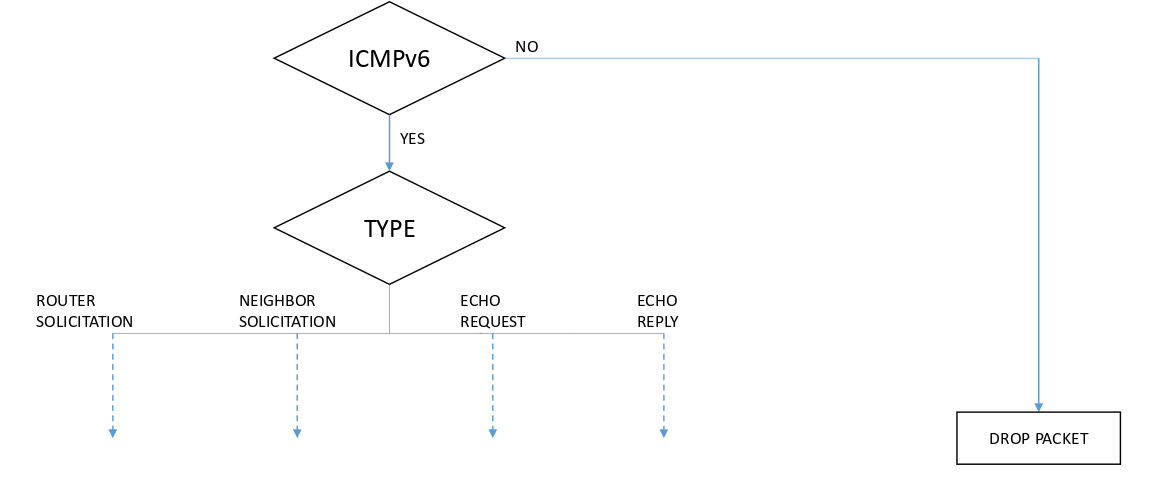
\includegraphics[scale=0.3]{reportPictures/controller_global_algo.png}
  \caption{Global algorithmic scheme of the controler}
\end{figure}

\subsubsection{Router Solicitation message}

The first type of message of a switch can receive is ICMPv6 Router
Solicitation message, this message is sent by hosts when they get their
interface turned on or when they access a new network.\\ 

\begin{figure}[h!]
  \centering
    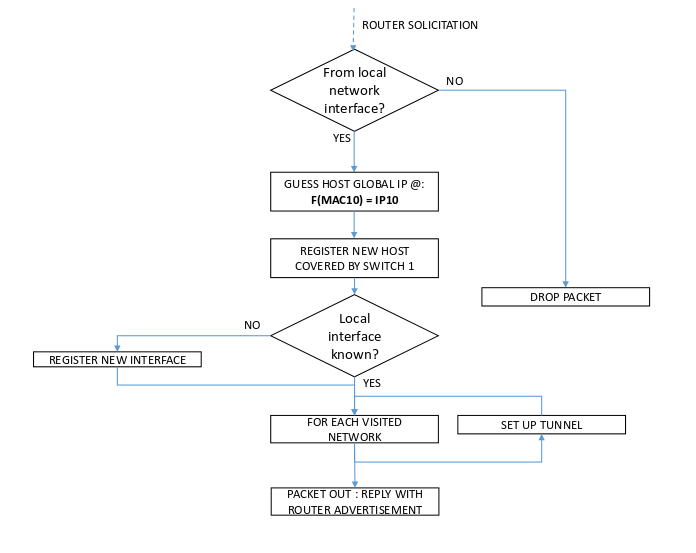
\includegraphics[scale=0.3]{reportPictures/router_solicitation.png}
  \caption{Controler algorithmic when handling router solicitation messages}
\end{figure}

What the controller does first in this case is checking if the input
interface of the switch is not already registered as backbone
interface, if it is the case, the controller does nothing. Otherwise
handling keep going and as now controller is sure that the source is a
host, it registers its MAC address (obtained from the source address
field of the frame containing the Router Solicitation Message) in a
data structure called coveredHosts. It stores hosts that have
registered inside the sub-network of each switch, in other words it
stores for each switch the hosts that are supposed to be linked to
it. This structure is a dictionary where keys are the couple: IPv6
addresses that the hosts has forged when joining the sub-network and
the identifier of the joined switch. Values are the couple host's
MAC address and the identifier of the switch's interface that is
linked to the host to make things clear hear is an example:\\ {dpid1
  : {host1IP:(host1MAC,intfLocal1),host2IP:(host2MAC,intfLocal2)} ,
  dpid2 : {host3IP:(host3MAC,intfLocal1)} }. \\
\newline
An important point is, since the host doesn't have any IPv6 address
yet, the one it generates from IPv6-autoconfiguration process is
guessed by the controller from host's MAC address and from the switch's
sub-domain in which the host is. It is important to have in mind that
if the host uses a different way to forge its Global IPv6 address, the
controller won't recognize it.\\
\newline
The bindingList is also extended, indeed if the Router Solicitation
message is received on an interface never used before, as the
controller just discovers it, it stores the new interface in the
coveredList: now its knowledge of the network topology gets extended
to local network interfaces and hosts to which they are linked.\\
\newline
Then as before an IPv6 address is assigned to this new discovered
interface and the controller has also a convention for local network
interfaces. The 2 bytes prefix of the address depends on the switch,
indeed switches define sub-domain among the network, but the first
half-byte of the prefix is always set to 2. Then the last two bytes of
the address is like before, defined by the interface number among the
switch. For example if the fourth interface of the switch number 7
through is linked to an host, interface's address is 2007::4.  If the
Router Advertisement reaches an already registered interface, nothing
happens on the bindingList.\\
\newline
This is just after this step that the mobility management is done,
the controller finds out if the host that has sent the Router
Solicitation message comes from another sub-network and triggers or
not mobility management procedure. For the moment we will skip this
part, considering first a controller that makes the network behave
normally, without any extra mechanism.\\
\newline
Last, the controller forges the ICMPv6 Router Advertisement to be sent
by the solicited switch to the host that just contacted it, it first
creates the core of the message this way: 

\begin{lstlisting}[frame=single,language=Python,breaklines=true ] 
icmp_v6 = icmpv6.icmpv6(type_=icmpv6.ND_ROUTER_ADVERT,
data=icmpv6.nd_router_advert(ch_l=64, rou_l=4,
options=[icmpv6.nd_option_pi(length=4, pl=64, res1=7, val_l=86400,
pre_l=14400, prefix=prefix)]))
\end{lstlisting}

with the variable 'prefix' set to the switch's local network interface
IPv6 address to which the host is bound. This packet is then
encapsulated in a IPv6 packet (with source address set to the local
scope address of the interface, generated on the fly like MAC
addresses) and in a Ethernet frame and is forwarded to the switch.\\ 
\newline
As we want every Router Solicitation messages to be reported by the
switches to the controller in order to keep track of hosts moves across
the network, no flow handling Router Solicitations messages are pushed
down to the switch but only a punctual order asking to forward the
provided Router Advertisement message on the specified interface.\\
\newline
Here is the associated code of a punctual order embedding a Router
Advertisement message (under pck\_generated name) sent by the controller
to the switch (called datapath here):

\begin{lstlisting}[frame=single,language=Python, breaklines=true] 
actions = [parser.OFPActionOutput(out_port)] 
out_ra = parser.OFPPacketOut(datapath=datapath,
buffer_id=ofproto.OFP_NO_BUFFER, in_port=0, actions=actions,
data=pkt_generated.data) 
datapath.send_msg(out_ra)
\end{lstlisting}

The switch will execute the given order in forwarding to the host the
Router Advertisement message and will keep reporting any Router
Solicitation messages coming next to the controller.\\

\subsubsection{Neighbor Solicitation message}

A second kind of ICMPv6 message that can be reported by switches to
the controller are ICMPv6 Neighbor Solicitation messages, there are
two reasons for an host to send such a message to its local switch. The
first one is in order to resolve the MAC address associated to a given
IPv6 address : the target address. In this case the option field of
the Router Solicitation message is not empty, and the controller
checks if the target address is one of the virtually assigned
addresses of the solicited switch's interfaces. If yes the controller
forges the corresponding Neighbor Advertisement message that contains
the IPv6 address of the spotted interface and transmits it back to the
switch along a forwarding order for being relayed to the host, exactly
as for Router Advertisement messages.\\

\begin{figure}[h!]
  \centering
    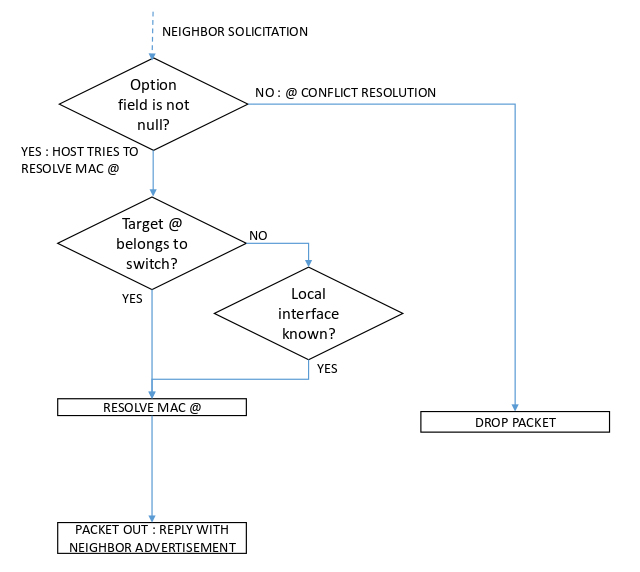
\includegraphics[scale=0.3]{reportPictures/neighbor_solicitation.png}
  \caption{Controler algorithmic when handling neighbor solicitation messages}
\end{figure}

As several hosts can be connected to the same switch and then get
configured with the same prefix even if they are linked to the switch
through different interfaces, the controller also resolves inside
domain requests : when a Neighbor Solicitation message received by a
switch has a target address corresponding to one of the hosts of
the local network. Then here, as every packet between hosts in the
sub-network goes through the switch, the packet containing frame built
by the sender will have its destination MAC address set to the MAC
address of the switch's interface it is linked to.\\
\newline
If the option field of the Neighbor Solicitation message is null that
means that it has been sent by the host for address conflict
resolution purposes, in this case, as address conflicts are not
considered, the controller doesn't do anything : all the host
registration process inside controller data structure is done at
Router Solicitation message reception.\\
\newline
As address conflicts are not handled by the controller, if an host
comes up with a new reconfigured IPv6 address it won't be recognized
by the switch since this address is not obtained from the usual IPv6
auto-configuration process.\\
\newline
Router Solicitation and Neighbor Solicitation messages are the only
two kinds of ICMPv6 control messages handled by the controller, as the
controller redefines itself the whole backbone addressing plan and as
address conflict is not managed there is no need to care about ICMPv6
Router Advertisement and Neighbor Advertisement Messages.

\subsection{ICMPv6 Echo request \& reply}

The last kind of message we want to be handled by the controller are
ICMPv6 Echo messages, they are representing data packets in the
simulation.\\
When the reception of on ICMPv6 Echo message is reported
by a switch to the controller, the controller first looks at packet's
destination address and behaves according to it.

\begin{figure}[h!]
  \centering
    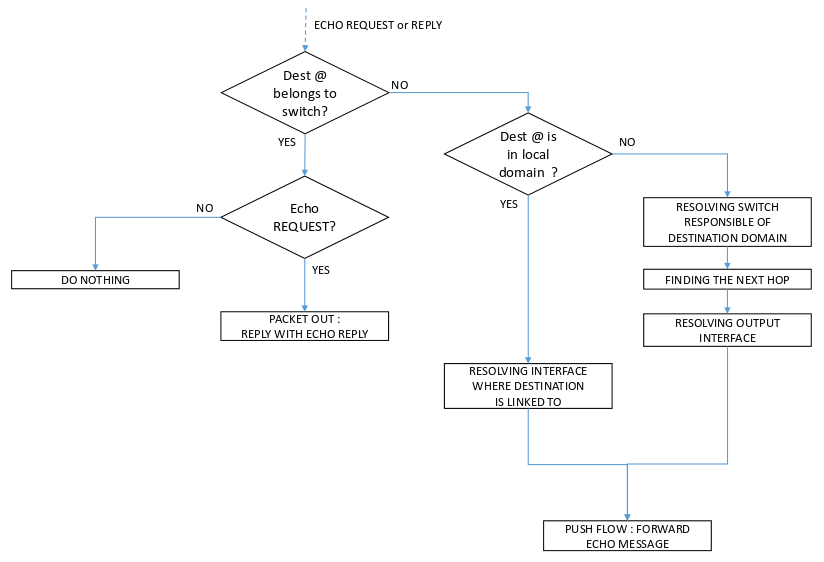
\includegraphics[scale=0.3]{reportPictures/echo_message.png}
  \caption{Controler algorithmic when handling echo messages}
\end{figure}


\subsubsection{Answering to Echo messages}
Once the controller gets packet's destination address it checks if
this address belongs to one of the interfaces of the solicited switch
using the bindingList, from which it retrieves switch's interfaces
this way:

\begin{lstlisting}[frame=single,language=Python, breaklines=true] 
localAddressesList = [ self.bindingList[localPort] for localPort in self.bindingList.keys() if localPort[0]==dpid ]
\end{lstlisting}

If the destination address is indeed one belonging to the switch,
there are two possible scenarios : if the message is an Echo Reply,
nothing has to be sent back to the network and the controller
doesn't do anything. If the message is an Echo Request, that means
that someone is pinging the switch then it has to reply.\\
\newline
Exactly as when the controller was ordering the switch to send a
Router Advertisement or a Neighbor Advertisement message, the
controller first constructs the ICMPv6 Echo Reply message and the
encapsulating packets, and pushes it to the switch along with a
punctual forwarding order toward the interface the Echo Request was
coming from.\\
\newline
Here we chose not to push flows to the switch since ICMPv6 Echo Reply
message is constructed from the associated Echo Request message, it
would have been necessary to push flows specific to each Echo
Request's destination address that have their specific
actions. Therefore flow table could have been over populated with Echo
message related flows which are not the interesting ones.

\subsubsection{Forwarding Echo messages}

When the destination address of the Echo packet is not one of the
solicited switch's addresses, that means the switch is one intermediate
node on the Echo message's path and have to forward it toward its
destination, regardless if its an Echo request or an Echo reply.\\
\newline
The controller then figures out what is the local network to which the
destination address belongs to: it extracts from the echo message's
destination address the number contained on its first two bytes. From
it, it gets the identifier of the switch the destination should be
linked to unless if it is a backbone interface that is aimed and the
result is null, in this case it extracts the last byte of the address
where is written switch's identifier.\\
\newline
Then two cases are possible, either the destination node is an host
directly linked to the solicited switch (in this case the extracted
identifier is the one of the switch itself) and here the controller
checks if there is an host registered in the coveredHosts list of the
switch that own Echo message's destination address. If no host is
found in the list the packet is dropped, but if one is found the
controller fetches host's details from the coveredHosts list that are
: host's MAC address and the switch's interface to which it's linked
to. With all of this the controller has everything he needs to make
the switch relay the echo message toward its destination.\\
\newline
If the extracted network identifier is not the one of the switch
itself: another switch or an host located in a remote local network is
aimed by the message. Here the controller finds out next hop switch
toward the destination : for this purpose is uses the structure called
networkGraph constructed during the initialization phase and runs on
it the breadth-first algorithm to get the shortest path between the
solicited switch and the destination switch. From the path, the
controller learns which switch is the next one to reach the final
one. The last step consists in, given a switch and one of its direct
neighbour, finding the interface of the switch that is linked to this
neighbor, the function routing() has been written for this purpose,
the idea is a to scans all the links of the network until finding the
one linking the two specified switches and look on which interface the
link is plugged on the switch, here is the code:

\begin{lstlisting}[frame=single,language=Python, breaklines=true] 
def routing(self, source, dest):
    for l in self.linkList:
        if l.src.dpid==source and l.dst.dpid==dest:
            return l.src.port_no
\end{lstlisting}

Since this function uses the linkList structure it only works with
interfaces linking one switch to another, that is why interfaces
linked to hosts are stored in the coveredHost structure.\\
\newline
When we reach this point in every cases we have resolved the switch's
interface on which the Echo message has to be forwarded. And as the
message has to be encapsulated in a new MAC frame, new source MAC
address and destination MAC address must be set. The source MAC
address depends on the switch's interface and is computed on the fly
as previously said, and the destination MAC address is fetched from
the coveredHost structure if the next hop is an host. If the next hop
is a switch the routing function is called on this switch in a
symmetrical way in order to resolve identifiers of the interface
located on the other side of the link. From it, the destination's MAC
address can be generated.\\
\newline
Now in every cases all the elements needed for forwarding have been
resolved (MAC addresses and Output interfaces) and here for the first
time a flow is pushed to the switch from the controller instead of
punctual order. This flow consists in matching every next Echo message
reaching the switch with the same destination address and to forward
them toward the interface that has just been resolved in changing MAC
address with the ones provided, here is the associated code:

\begin{lstlisting}[frame=single,language=Python, breaklines=true] 
action =
[parser.OFPActionDecNwTtl(),parser.OFPActionSetField(eth_src=new_mac_src),
parser.OFPActionSetField(eth_dst=new_mac_dst),parser.OFPActionOutput(outputIntf)
]
match = parser.OFPMatch( eth_type=0x86dd, ip_proto=58, ipv6_dst=(ping_dst,'ffff:ffff:ffff:ffff:ffff:ffff:ffff:ffff'))
self.add_flow(datapath, 1, match, action,tblId=1)
\end{lstlisting}

Now the switch knows how to handle alone this specific kind of message
and won't forward it anymore to the controller. This is how switches
get progressively autonomous, by getting instructed at each reception
of a new Echo message to forward.\\
\newline
Now the controller is able to handle switches over a normal network
that is not requiring any extra services, but our purpose is to handle
host mobility over the network, then we can imagine that other flows
will be pushed down to switches so it is necessary to organize flows
properly into switches order to avoid any conflict between flows of
different purposes.

\section{Handle host mobility across the network}

\subsection{Introduction}

\subsubsection{Flow organization inside switches}
Once pushed to a switch, flows are grouped into ordered tables that
can be bound together, our controller defines 3 tables insides
switches : the first one (table number 0) and the last one (table
number 2) are dedicated to flows related to mobility handling and
their purpose will be explained later, for the moment the only thing
to know about them is that the default entry policy of table number 0
is to forward message to the table number 1.\\
\newline
The table number 1 (the second one) is dedicated to flows related to
classic message forwarding, like the flows pushed for relaying ICMPv6
Echo messages. At this point tables 0 and 2 are empty and the second
one get progressively populated witch flow associated to Echo messages
forwarding. For each switch, when a packet is received, it checks if
it matches one of the entries of the first table, if not it checks if
it matches one of the entries of the second table. If no match is
found after having scanned the second table, the switch doesn't know
how to handle it and asks the controller what to do with it (it's
asking for an order or a new flow), that is what happens when a Echo
message with a new destination reaches the switch.

\subsubsection{Basic idea of how mobility management is done}

Host mobility is ensured first in keeping track of them all around the
network, by storing and updating the list of sub-networks each node
has visited. So that when a host gets to a new network, all the old
ones registered on the list are retrieved and involved in the mobility
management procedure.

\subsection{Retrieving Mobile Host history and enable local forwarding}

\subsubsection{Retrieving Mobile Host history}
When a Router Solicitation is submited to the controller, after it has
updated coveredHosts and bindinList data structures, the controller
refers to the module called mobilityPackage to know if the host has
visited sub-network before connecting to the solicited switch. This
module is very simple consists in one dictionnary called trackingDict
which stores the network history for each host and provides a unique
function called getTraceAndUpdate(), that returns the list of
previously visited networks by a specific host identified by its MAC
address and appends to this list the identifier of the switch which
notifies the Router Solicitation message to the controller.\\
\newline
The controller next build a tunnel between each previously visited
returned by the module and the solicited switch which is now the one
to which the mobile host is linked to, and therefore the one to which
all the mobile host's on going communications has to be re-routed.

\subsubsection{Enabling local forwarding of remote addresses}
When a host gets connected to a switch, the controller computes the
Global IPv6 address the host will generate and stores it into the
coveredHost data structure so that when a ICMPv6 Echo message is
aiming this particular address the controller can resolve the
interface to witch the host is linked and the Echo message can be
forwarded.\\ 
\newline
When now the host has visited other networks before connecting to a
new switch, by setting up tunnels the controller makes all the active
communications in which the host is involved, going through the new
switch. Then, in this case the new switch receives packets coming from
everywhere in the network and has to forward them on the interface the
mobile host is now linked to. Since those communications have been
started by the host other sub-networks, they are made of packets for
which the host address is a previously generated one and the new
switch doesn't have any ideas of them. Therefore to be able to achieve
correctly the local forwarding, the switch has find out which are
those previous addresses used by the host so that output interface can
be resolved.\\
\newline
A simple solution to this issue consists in first resolving the
previously IPv6 addresses used by the host and then pushing new flows
from the controller to the new switch's table number 1 (the table for
routing purposes) that would match packets whose destination address
is the ones just resolved and forward them on the interface where the
host registered. The problem now is that some packets that doesn't
come from any tunnel may be forwarded to one of the new switch local
interface instead of being routed normally, the switch associated to
their destination address. Therefore those new flows would mess up the
normal routing procedure and we want to keep this very particular
local forwarding of remote addresses only for packets coming from
tunnels and keep other packets out of it.\\
\newline
That is why a third flow table is set up inside switches, it contains
all the flows related to local forwarding of remote address. The
important point is that flow table can only be accessed by messages
coming from a tunnel. As host's previous network are known as well as
host's MAC address, the controller computes the global IPv6 addresses
the host has generated when it was in those networks, and then pushes
flows that match packets having those addresses as destination address
and make the new switch forward them on the interface on which the
Router Solicitation message has been received.

\subsection{Setting up tunnels}

\subsubsection{General scheme}
Tunnels are established between the switch just joined by the Mobile
Host and the ones it was connected to before. In this way all the
messages aiming an address that the host has forged in a old
sub-network reach the associated router that forwards them in the
tunnel just set up to the new switch that extract them out of the
tunnel and relays them to the host.\\ 
\newline
In the reverse direction, when the host sends a message with a old
generated IP address as source address, this message is tunneled from
the new switch to the one covering the sub-network where this old
address has been built (no route optimization mechanisms are set
up). The old switch then extract packets out of the tunnel and
forwards them toward their final destination.

\subsubsection{Tunnel properties}

Tunnels are materialized with Vlan tags, as it only deals with the
layer 2 of switches' stacks, the handling is lighter and faster for
them.\\ 
\newline
Moreover for a given direction, only one tunnel exists between
two switches and it is shared between hosts, this makes the number of
flows to push for mobility purposes lower, indeed, the first host that
goes from a network A to a network B will trigger the establishment of
a tunnel between the associated switches and every next host that do
the same crossing from A to B will have its message going conveyed
through this same tunnel.\\ 
\newline
Tunnels are unidirectional on the way hosts move, in the sense that
they convey messages (in both directions) to ensure host mobility from
a network A to another network B but if the host goes back to A from B
another tunnel will be used. Indeed it is not possible to merge two
opposite tunnels into one as switch's job is not the same when the
switch is on the new or on the old side of the tunnel.

\subsubsection{Tunnel related flows}

A tunnel between a previously visited switch A and the currently
visited switch B is set up by the controller first in pushing two
flows to both switches A and B. This time flows are related to host
mobility, they are then store in the first table (table 0) of each
switch.\\
\newline
Two flows are pushed to the first table of switch A:\\
\newline
The first one matches packets coming from the network whose
destination address is the one that the Mobile Host forged when it
was in the sub-network of switch A (let's call this address
"host's old address"), and its action consists in pushing a VLAN
tag on those packets, and forwarding them toward router B, in
changing MAC addresses. Here the VLAN tag is the concatenation of
switch A and switch B's identifiers (let call this value "V"). To
avoid any undesirable tunnel binding effect the flow matches only
packets without VLAN tag.\\
\newline
The second flow matches packets whose source address is the host's
old address and which include a VLAN tag set to V. The
associated action consists in first getting rid of the VLAN tag
and then in relaying the new packet to the flow table number 1 of
the switch so that it will be passed through the table like a
normal packet from the local network and be forwarded as usual to
the external network.\\
\newline
Two other flows are pushed to the first table of switch B:\\
\newline
The first one matches all the received packets whose source address
is the host's old address. The associated action is to push a VLAN
tag with the value V and then to forward packets toward router A,
in changing MAC addresses. As IPv6 addresses are unique there is
no risk that this flow matches packets received on a backbone
interface of switch B and forwards them into the tunnel because
the mobile Host is the only entity of the network that sends
packets with this precise source address. Here again, to avoid any
undesirable tunnel binding effect the flow match only packet
without VLAN tag.\\
\newline
The second flow matches packets from router A that include a VLAN
tag set to V, then the associated action consists in first
stripping the VLAN tag out of packets. Second, as those packets
have their destination address set to the host's old address they
are then relayed to the flow table number 2 of switch B so that
the local output interface will be resolved based on the
destination address of the packets.\\
\newline
Now that flows are pushed to the entry point and to the exit point of
the tunnel, the controller has now to tell switches of the network
this tunnel crosses to relay packets going through the tunnel. In
applying the breadth-first algorithm over the networkGraph data
structure, the controller gets the list of the intermediate switches to
instruct, and push to each of them two flows : \\
\newline
The first one matches packets that include a VLAN tag set to V and
whose source address is host's old address, the associated action is
forwarding them in keeping them unchanged (except their MAC
addresses) to the next hop on the path to reach B.\\
\newline
The second one matches packets going in the reverse direction, those
ones include a VLAN tag set to V and their destination address is host's
old address, the associated action is forwarding them in keeping them
unchanged (except their MAC addresses) to the next hop on the path to
reach A.\\
\newline
With this set of flow host mobility is ensured all over the network
but there is currently one configuration that makes the program not
working : when the tunnel entry point has to forward encapsulated
packet on the same interface on which it has received them just before,
it doesn't forward anything out on the interface and nothing is send
inside the tunnel. This problem is not fixed today!

\subsection{Advanced mobility}
It's important to keep in mind that the mobile host may not only go
from one network to another but may roam across many different ones
and also go back to previously visited networks. Therefore the tunnel
establishment algorithm described before is a trade between having a
simple sequence of operations to be done by the controller and try not
to make switches flow table soaring after host have roamed for a
while, that is why shared tunnel solution has be selected.

\subsubsection{Subsequent Handover}

When the mobile host, after having left its home network A to go to
network B, changes again of network and goes to network C, there are
now two address for which mobility have to be ensured : the one
acquired in network A and the one acquired in B, that means that two
tunnels have to be set up : one between switch A and switch C and
another between switch B and switch C, moreover the previously tunnel
from A to B must not be used anymore for the considered host.\\
\newline
 Once installed into a switch, a flow can be updated when a new flow
with the same matching criteria is pushed to this switch, this is
what happens when the host gets to network C. Before the host joins
switch C, two tunnel flows are installed into switch A : one ensures
that every packet aiming the mobile host's old address is forwarded in
a Vlan tunnel toward B, let's call this flow FA1. The other one
ensures that every packets going from the Vlan tunnel is piped to the
routing table, let's call it FA2.\\
\newline
When the mobile node reaches network C, a new Vlan tunnel is set up
between switches A and C, FA1 is then updated because a new flow
matching every packets aiming mobile host's old address forged in
network A is pushed, and this new flow makes switch A forwards them
into the new Vlan-tunnel toward C. From now switch A doesn't forward
anymore packets related to the considered mobile host in the tunnel
it shares with switch B (but it still can forward into it packets
related to other mobile hosts). The second new pushed flow matches
packets based on a new Vlan tag, then it doesn't update FA2 as tunnels
between A and B and between A and C use different tags. \\
\newline
Then switch A has now 3 flows in its flow table number 0 : two of them
handle host mobility toward network C and the last one is now useless
for the considered host but still important to handle mobility of
other mobile nodes that have moved from network A to network B.\\
\newline
The two new flows pushed to switch B when the mobile node gets in
network C are exactly analog to the ones pushed to switch A when the
host moved from network A to network B, but they are associated with
the new Vlan tunnel between switch B and switch C. One of the two
already existing flows related to the Vlan tunnel established with
switch A, was in charge of forwarding packets coming from the tunnel
to switch B's flow table number 2, let's call it FB1. The other one
was matching packets with the mobile host's old address as source
address and was sending them into the tunnel, let's call it FB2. As
the mobile node is not anymore in network B, FB2 becomes completely
useless as the mobile host is no more emitting directly toward switch
B, but FB1 is still used for other mobile nodes that have moved from
network A to network B.\\
\newline
Two pairs of flow are then pushed to switch C they are analog to the
pair pushed to switch B when the mobile node reached network B from
network A, but one pair is related to the tunnel between switch A and
switch C and the other to the tunnel between switch B and switch C.

\subsubsection{Subsequent Handover Complexity}

In this scenario of subsequent handover, when the node gets to network
C, 8 flows are pushed by the controller, and every time a mobile node
moves to a new network, n time 4 flows will be pushed with n the
number of visited networks. Indeed the fact of having simple flow
pushing algorithm makes the number of OpenFlow messages quite
important. However, our method doesn't present a great space
complexity regarding to switches flow tables, and especially for the
first flow table. Indeed as tunnel are shared, among the four flows
pushed during the first handover between network A and network B, one
(FA1) is updated, two are still useful for other mobile hosts (FA2
and FB2), and only one becomes unused (FB1) until the mobile node
goes back to network B.

\subsubsection{Back to a visited network}

If the mobile host, after having visited network C, keeps roaming and
goes back to network B, the mobility of the the address acquired in
network A and of the one acquired in network C have to be ensured,
moreover packets going to the address that the mobile node has forged
in network B doesn't have to be transferred in a tunnel anymore.\\
\newline
First, two flows are pushed to switch A and two others are pushed to
switch B and as they are exactly the same as the one pushed when the
host moved first from network A to network B (the Vlan tag is still
the same), there won't have new flows in switch A and switch B's flow
table but the flow FA1 will be once again updated and incoming
packets aiming the host's old address forged in network A will be
forwarded to the tunnel toward B.\\
\newline
Two other pairs of flow are pushed to switch C and switch B again,
indeed as we said tunnel are unidirectional in the sense that one
tunnel ensure mobility between two switches for a given direction, then
two more entries are written in both switch B and switch C's flow
table.\\
\newline
Packets going to the address that the mobile node forged into network
B when it got there for the first time were matched by a flow entry
that sent them into the tunnel between switch B and switch C. Now
this flow entry is updated by the controller that pushes a last flow to
B with the same matching criteria and that forwards packets on the
second flow table of switch B, so that packets going to this specific
address are forwarded normally by B toward the local interface the
mobile Host just connects to. \\
\newline
When the mobile nodes goes back to a previously visited network, old
flow entries are used again, and then flow table size doesn't become
very high. As each mobile node is associated to the list of the
networks that he visited, if it goes back to previous networks, the
same network indentifier can occur multiple time on the list, then in
order to avoid to push multiple times flows related to the same tunnel
during the same handover procedure, the controller keeps in memory
which tunnel it has already updated in order not to send new flows
related to an already updated tunnel.\\
\newline
\section{Observations and results} 

\paragraph{Introduction}
This part is following the steps of what is supposed to be presented
during the final presentation, its role is to illustrate and make
clearer the concepts presented in the previous section.

\subsection{Network topology and simple ping}

\subsubsection{Topology}
Let's consider a network composed by five switches and six hosts,
organized according to the following scheme : 

\begin{figure}[h!]
  \centering
    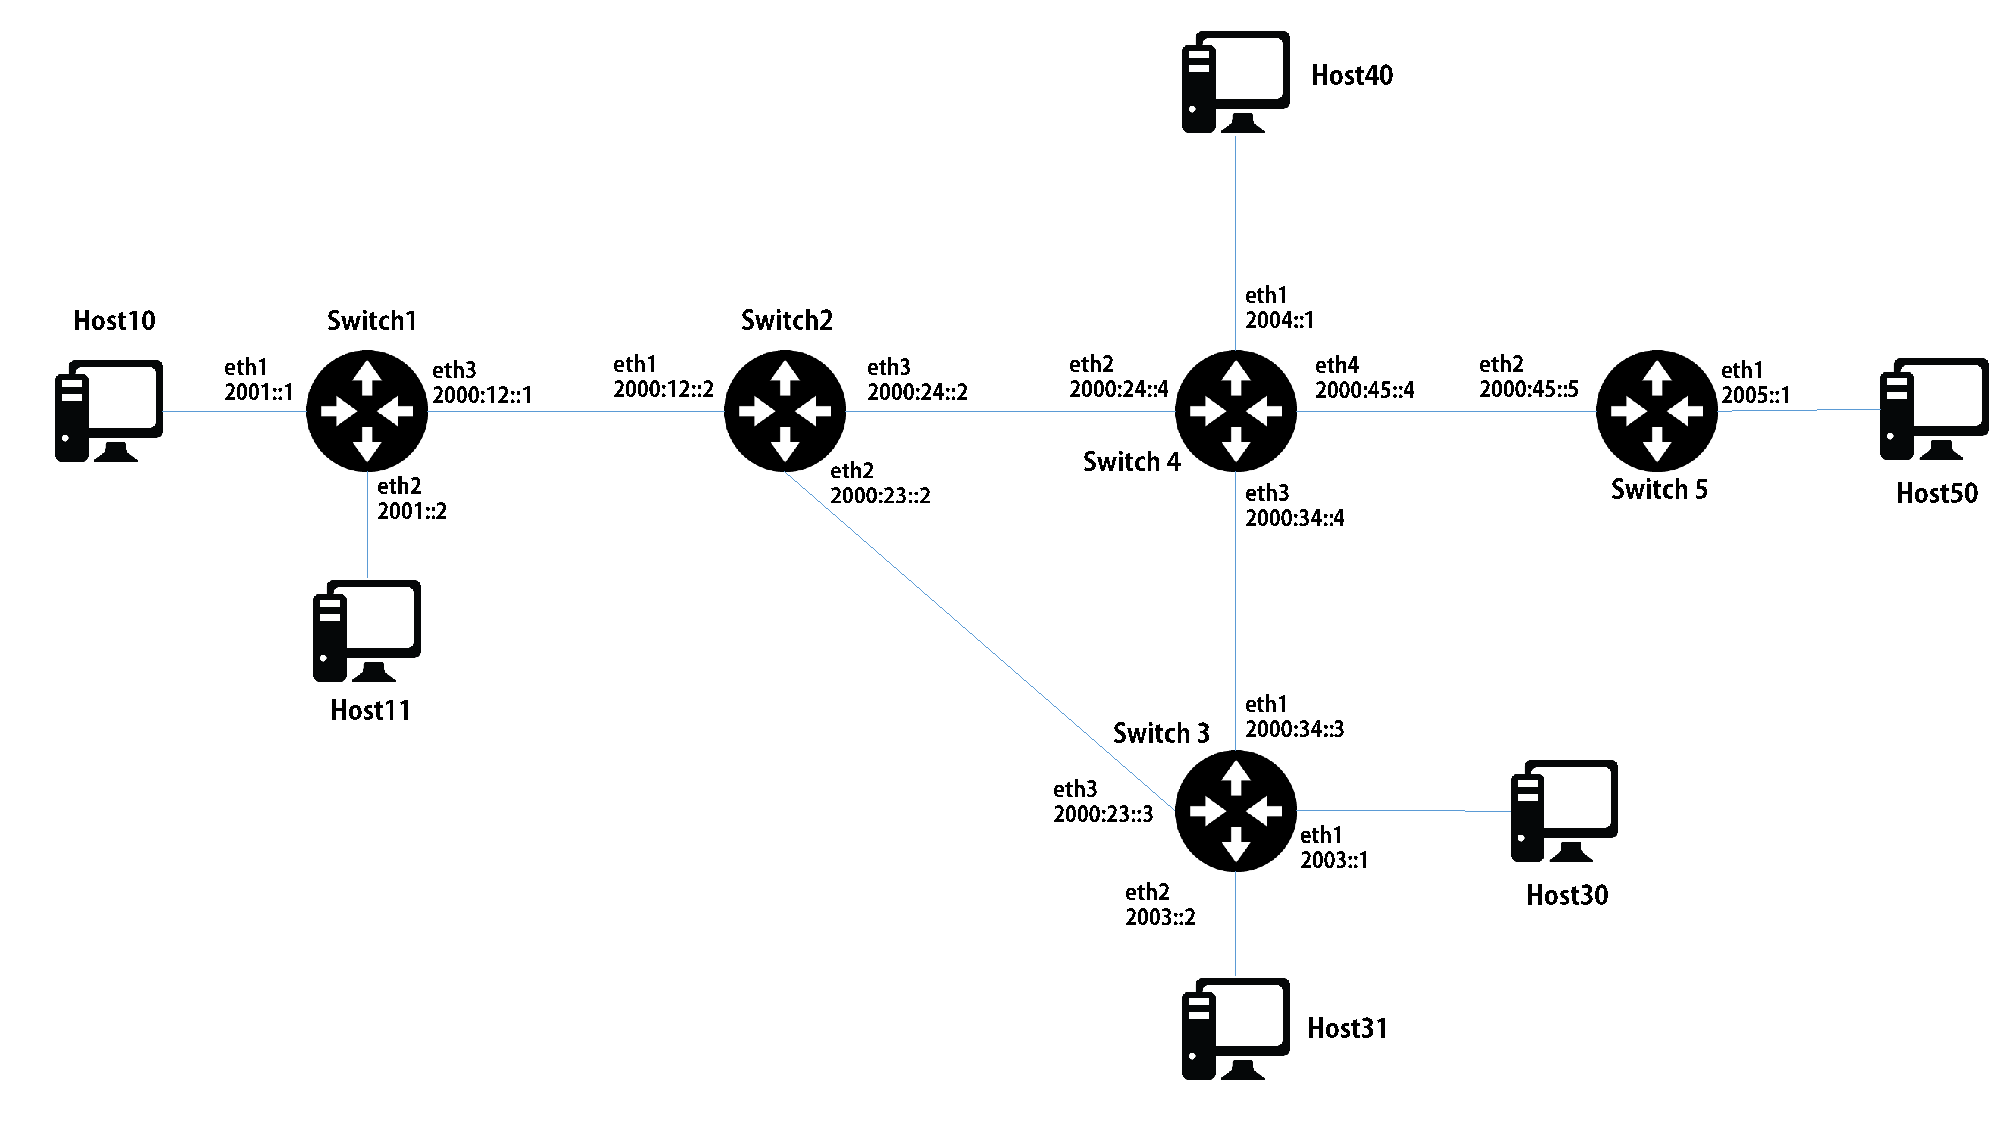
\includegraphics[scale=0.3]{reportPictures/networkmap.pdf}
  \caption{Network topology and addressing}
\end{figure}

\newpage

A mininet script has been written to reproduce this topology, to make
things clearer the script assignes to each switch address that will be
virtually generated by the controller. It also makes the default route
configuration on hosts easier.\\
\newline
Once both mininet and the controller are launched, after few seconds
hosts get configured with global IPv6 addresses, here is a view of
h10's interface configuration:

\begin{figure}[h!]
  \centering
    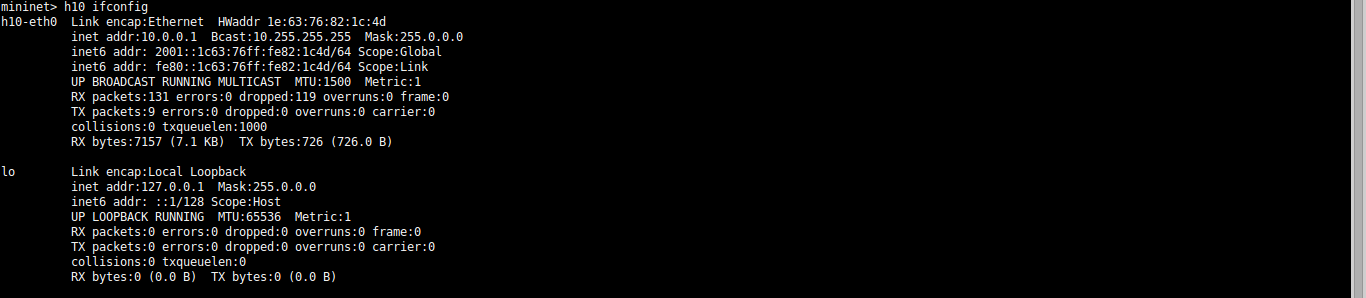
\includegraphics[trim = 0mm 0mm 237mm 0mm,clip,scale=0.5]{reportPictures/h10_autoconfiguration.png}
  \caption{Interface configuration of h10}
\end{figure}


\subsubsection{Simple Ping}
To enable hosts to send messages, they have to be given a default
route, here the local router is the default route.\\
\newline
From now hosts are able to ping each other, the first ping messages
won't be conveyed to their destination as flows are getting pushed
to switches but once they received all the information from the
controller, messages are well relayed. Here is an example with h10
pinging h31's IPv6 address : 

\begin{figure}[h!]
  \centering
    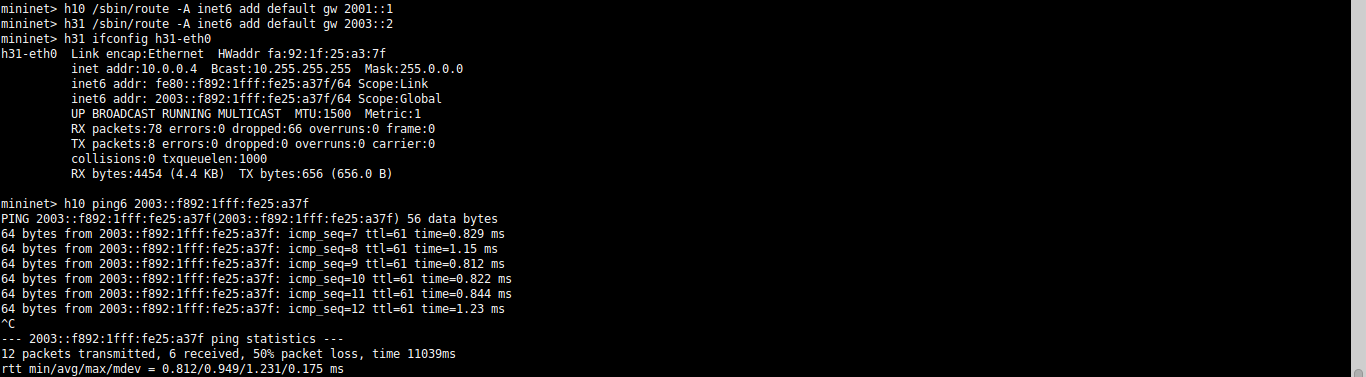
\includegraphics[trim = 0mm 0mm 237mm 0mm,clip,scale=0.5]{reportPictures/h10_ping_h31.png}
  \caption{Ping messages between h10 and h31}
\end{figure}


The first message of this series of ping has triggered flow pushing to
the second flow table of switches on the path from h10 and to h31, at
the beginning those tables were empty and now they get populated with
the occurrence of new ping messages, here is the content of the flow
tables of s1.

\begin{figure}[h!]
  \centering
    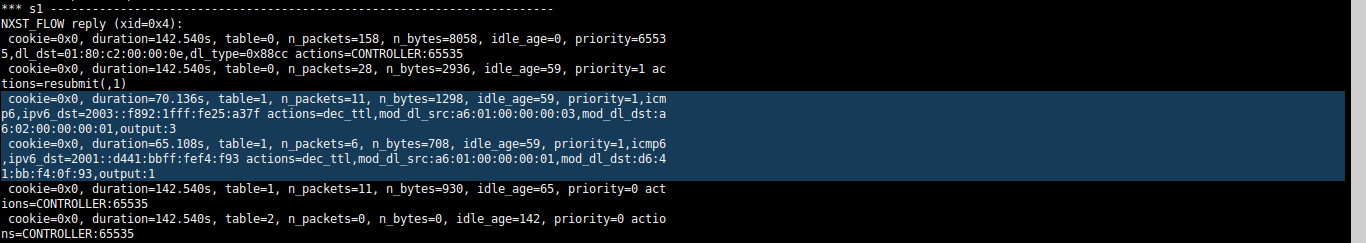
\includegraphics[trim = 0mm 0mm 237mm 0mm,clip,scale=0.5]{reportPictures/s10_dumpflows.png}
  \caption{Flow tables of s1}
\end{figure}

At this moment the two other tables are still empty.

\subsubsection{Simulating one hop mobility}

As making hosts move from one router to another with mininet looks
possible to implement in a python script, but not with command line
instruction. The idea to overcome this issue is to use IP and MAC
spoofing inside the network. Indeed let's configure h50 with the same
addresses as h31 while h31 is turned off, as h50 presents h31
identifiers the controller will treat it as if it was h31.
Here are the spoofing instructions: 

\begin{figure}[h!]
  \centering
    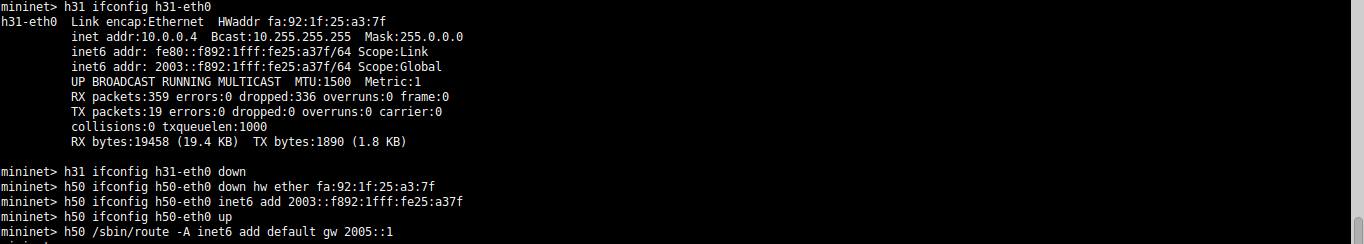
\includegraphics[trim = 0mm 0mm 237mm 0mm,clip,scale=0.5]{reportPictures/h50_spoofs_h31.png}
  \caption{Spoofing instructions}
\end{figure}

Now, if h10 pings again h31's address, ping messages are still well
exchanged but now the TTL of the ping response is equal to 59 whereas
it was equal to 61 before, that means that there is two more hops now
on the path from h10 to h31's address. With a packet sniffer it is
possible to see ping messages going from s1 to s3 and then being
relayed in VLAN tagged packet to s5, h31's address mobility is then
provided.

\begin{figure}[h!]
  \centering
    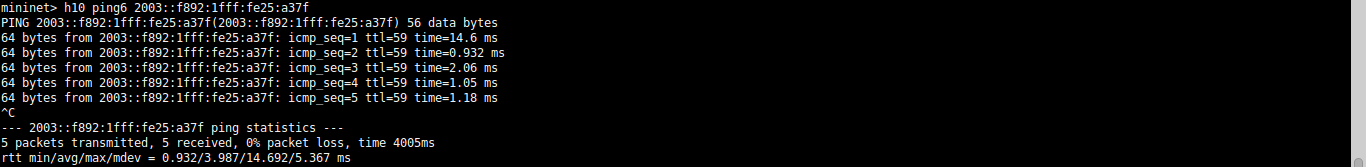
\includegraphics[trim = 0mm 0mm 237mm 0mm,clip,scale=0.5]{reportPictures/h10_ping_h31spoofed.png}
  \caption{ping message between h10 and h50 spoofing h31}
\end{figure}


Ping messages are now received and treated by h50 that now plays the
role of h31 as we can see from a packet capture on h50's interface:

\begin{figure}[h!]
  \centering
    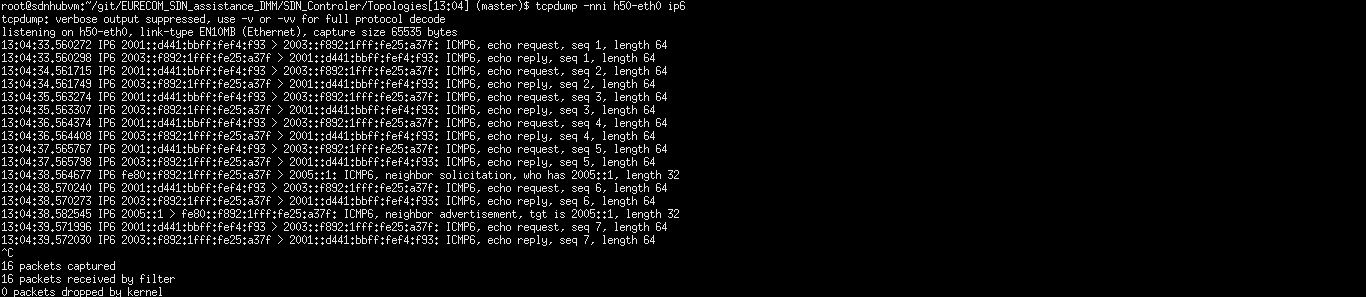
\includegraphics[trim = 0mm 0mm 237mm 0mm,clip,scale=0.5]{reportPictures/h50_tcpdump.png}
  \caption{Capture of ping messages on h50 interface}
\end{figure}

Flow tables have been updated, the first flow table of s3 is now
containing two flows that transfer packets going to h31's address in
the tunnel toward s5. The first and third flow table of s5 have
also been populated as we can see:

\begin{figure}[h!]
  \centering
    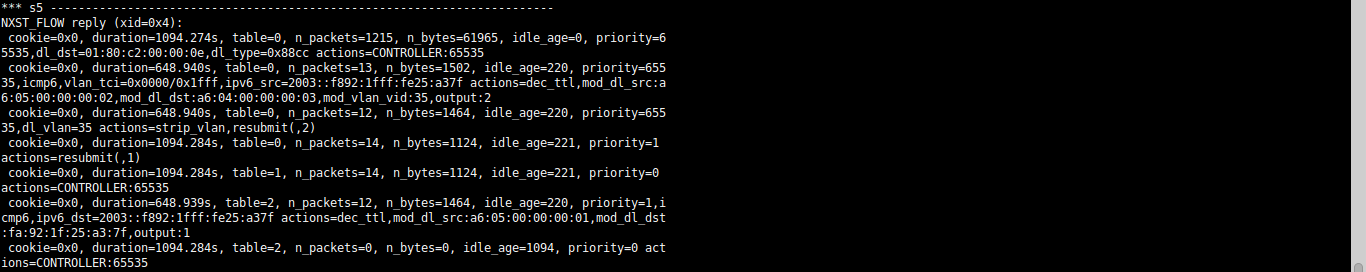
\includegraphics[trim = 0mm 0mm 237mm 0mm,clip,scale=0.5]{reportPictures/s5_dumpflows.png}
  \caption{Flow tables of s5}
\end{figure}

\newpage

\subsubsection{Simulating advanced mobility}

Let's now turn h50 off and make h40 impersonate h31 exactly as the same
way we did before with h50, the controller will then believe that h31
has now moved from s5 coverage to s4 coverage.  Then ping messages go
now through a new tunnel between s3 and s4, and second tunnel is set
up between s5 and s4, we can retrieve them with the dump of s4 flow
table:

\begin{figure}[h!]
  \centering
    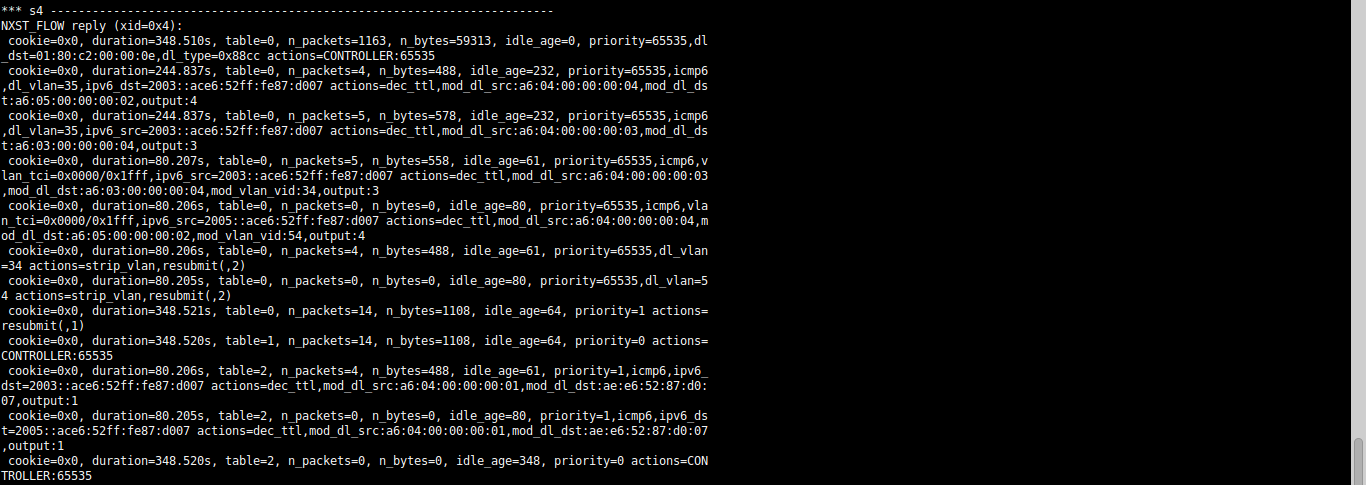
\includegraphics[trim = 0mm 0mm 237mm 0mm,clip,scale=0.5]{reportPictures/s4_dumpflows.png}
  \caption{Flow tables of s4}
\end{figure}


When the mobile node moves back under s3 coverage after having
visited s4 network, flow tables are updates and ping messages are now
routed again to s3 and s3 now forwards packets going to h1'address
not anymore on a tunnel but on its local interface where is now
plugged h31.


\part{Conclusion \& Futur Enhancements}

\section{Conclusion}

We have finally managed to implement a controller working regardless
the underlying network topology and built for IPv6. Simulation shows
that host mobility is well handled then now controller code can be
tested on a physical network. This controller can be also used only for
managing classic IPv6 network without host mobility needs.\\
\newline
This project has been a great opportunity to work with Software
Defined Networking tools and to understand deeply the concept. It has
also been a great mean to discover the latest frameworks built for SDN
and the details of OpenFlow.

\section{Enhancements}

\subsection{Controller algorithms}

\subsubsection{Having less flow to push}
We already said that each time a node moves to a new network after
having visited n networks, 4 time n flows have to be pushed down by
the controller, then after a while it can turns out to be lot of flow
to send. In order to limit this number a new way to handle mobility
would be only to set up a tunnel between the switch of the network
just left by the host and the one of the network just reached, then
mobility would be ensured with this series of tunnel bound one after
the other one among which switches would forward packets going to the
address the mobile node has forged under their coverage but also
packets going to the address the mobile has forged in the network
visited before : coming from the sequence of tunnel.

\subsubsection{Handling the first packets of flow}
As routing flows are pushed re-actively the first packets of a sequence
that triggers a flow pushing are lost. This can be avoided in
implementing a buffering mechanism inside the controller or in making
it tell switches to forward those packets to their destination
while flows are being set up.

\subsubsection{Handling other types than ICMPv6}
Flows pushed to both the first or the second flow table of each switch
match IPv6 echo messages, this has to be changed in the future
to allow other types of message to be treated. The question then is
gather all the network traffic type in one general matching flows or
assign specific flows for each supported protocol.


\subsubsection{Handle address conflict within the same sub network}
In our implementation, we suppose that hosts compute their local and
global IPv6 addresses following an unique method implemented in the
controller. Address conflicts between hosts leading to a different
manner to forge them are then not considered by the controller.

\subsubsection{Introducing access control to mobility service}
As mobility management is presented as a service it would be nice to
control which user can use it. Then the implementation of a policy
decision an enforcement entity could be done which would be consulted
when a new user shows up in the network. The authentication can be
first based on the mac address, and then on more advanced criteria. 

\subsection{Interaction with Mininet}

\subsubsection{Make hosts move for real}
Yet a way to make host moves from one switch to another within the
Mininet virtual network hasn't been found, that is why our way was to
trick the SDN controller with addresses spoofing. But as hosts doesn't
properly move in our simulation we do not really know how the system
really reacts and may be the messages exchanged between the mobile
node and the switch are not exactly the same.

\subsubsection{From command line to a batch program}
Our demonstration has been done in typing one by one all the Mininet
instructions that turns out to be quite the same, it would make the
interaction with Mininet easier and faster especially during the test
phases to load once an instruction file instead of writing them all
every single time. 
 
\subsection{fixing the bug}
When a ICMPv6 Echo message has to be forwarded by a switch on the same
interface that it has been received, nothing happen : the flow that
tell the switch to forward the packet is matched but the output packet
is not detected by packet sniffer. This problem even occurs when
packets to forward are modified in getting inserted a Vlan tag in
their structure. Then tunnel establishment is strongly impacted by
this bug whose origin is still not known.

\end{document}
